\chapter{Results and Interpretation}

%%%%%%%%%%%%%%%%%
%     2016
%%%%%%%%%%%%%%%%%
\section{2016 Datasets}

\subsection{Primary Analysis}
In order to roughly understand a group (similar patterns) of data, one way to do it is to reduce the dimension of data. In our case, there are 259 features which will be transformed into two-dimension on the basis of two eigenvectors (selected by two largest eigenvalues) belonging to covariance matrix which computed from the datasets.
\begin{figure}[h!]
    \centering
    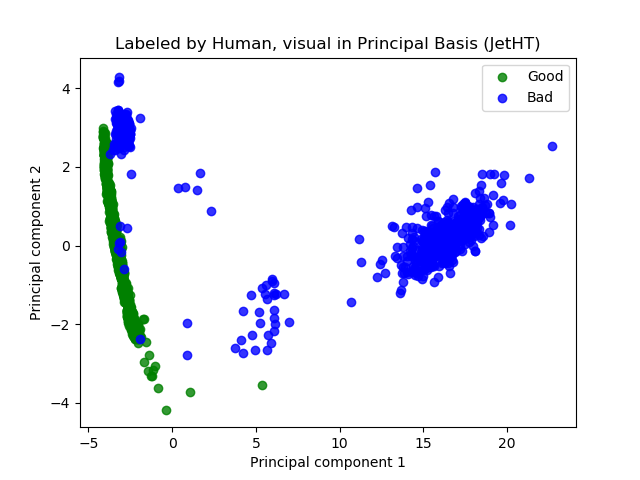
\includegraphics[width=0.6\textwidth]{images/reco/2016/JetHT_label_2016.png}
    \caption{Principal component with the labeled color from the system}
    \label{fig:JetHT_label_2016}
\end{figure}

As it can be seen on the green line in Figure \ref{fig:JetHT_label_2016} that there are nice band which is good LS and a few weird LSs that located outside the tubular shape as well as bad LS that could be divided into the bad LS with some patterns and anomaly bad LS which I would call both of them as "outlier". That's essentially the punchline why I called outlier detection instead of anomaly detection.

\subsection{Performance}
By Iteratively retrain the model ten times to make sure that it's working systematically and plot the root mean square as a shady fluctuation in Figure \ref{fig:performance_2016}
\begin{figure}[h!]
\centering
    \begin{subfigure}[b]{0.49\linewidth}
        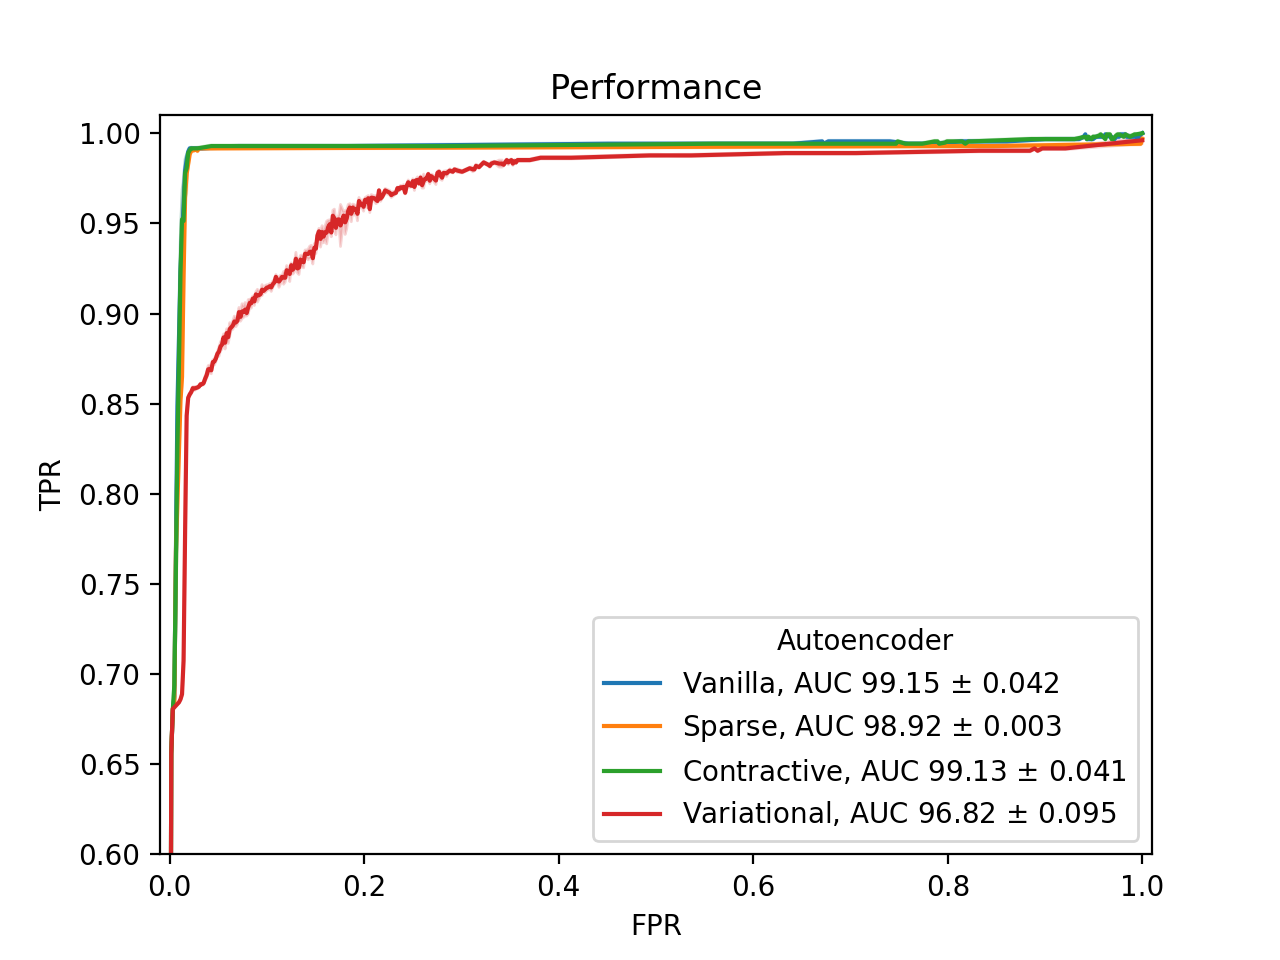
\includegraphics[width=\linewidth]{images/reco/2016/performance.png}
        \caption{4 Flavours of AE}
    \end{subfigure}
    \begin{subfigure}[b]{0.49\linewidth}
        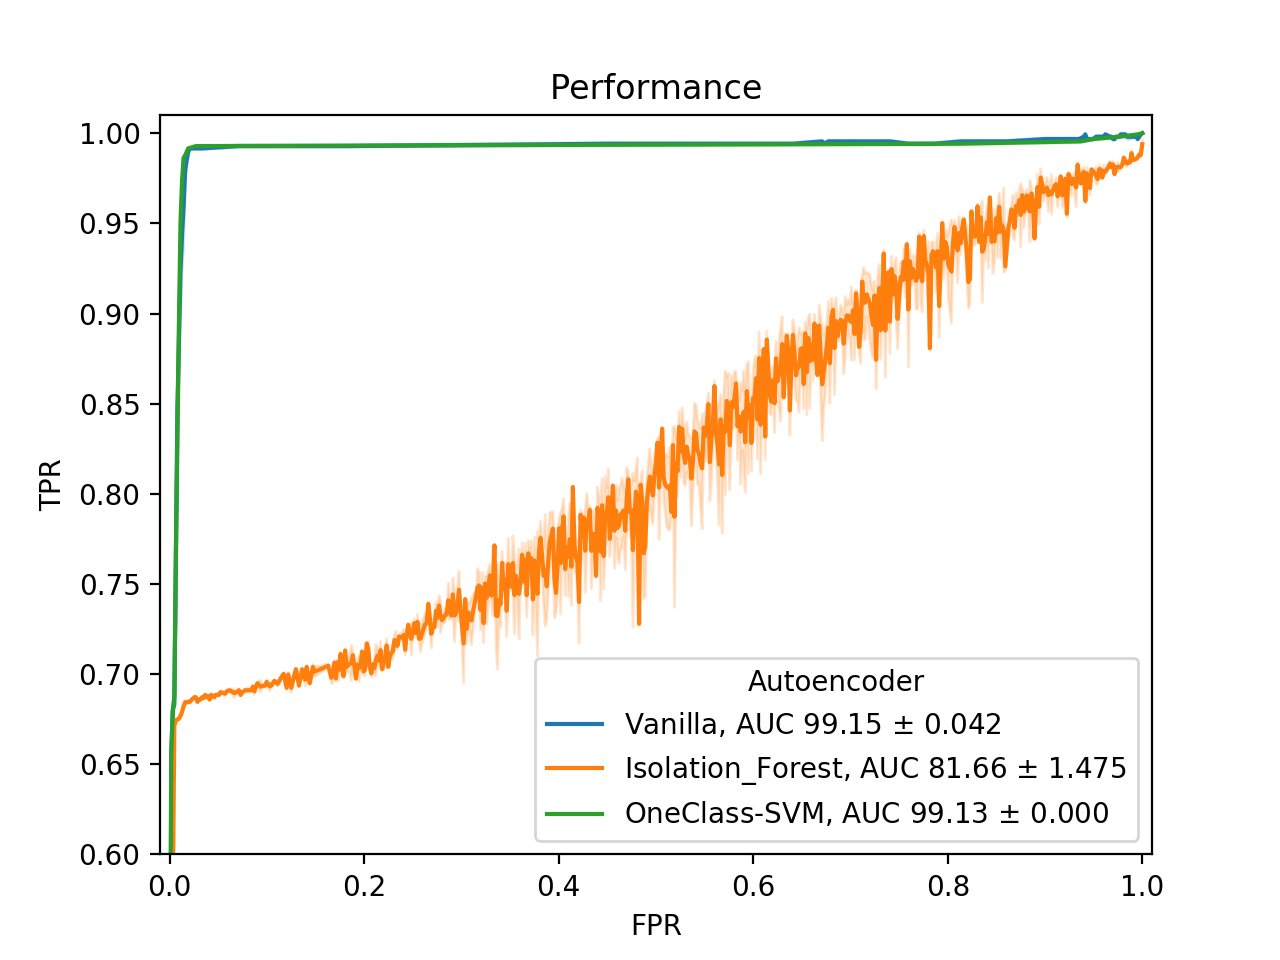
\includegraphics[width=\linewidth]{images/reco/2016/performance_ml.png}
        \caption{Vanilla AE vs SVM vs Isolation Forest}
    \end{subfigure}
\caption{Comparative visualization of model performance}
\label{fig:performance_2016}
\end{figure}

To sum up, even there are a fancy mathematical expression of non-vanilla autoencoders but it does not guarantee that we would get the best performance out of it. On the other hand, the simplest AE has the performance among all AE. One other interesting spot is the performance of OneClass-SVM also yields the remarkable results as nearly compatible with Vanilla AE without any fluctuation since the model itself has no randomness and work very straightforward.

\subsection{Distribution of decision value (to find the threshold)}
The story behind the performance figure is genuinely extracted from the distribution of decision value from Figure \ref{fig:2016_decision_value_dist} and slowly moving a threshold of minimal point in the overlapping region of good and bad LS from a label in the distribution until it got the maximal value. The below figures are the comparison between our two great candidates by considering to pick some threshold and see the contamination on each side.

\begin{figure}[h!]
    \centering
    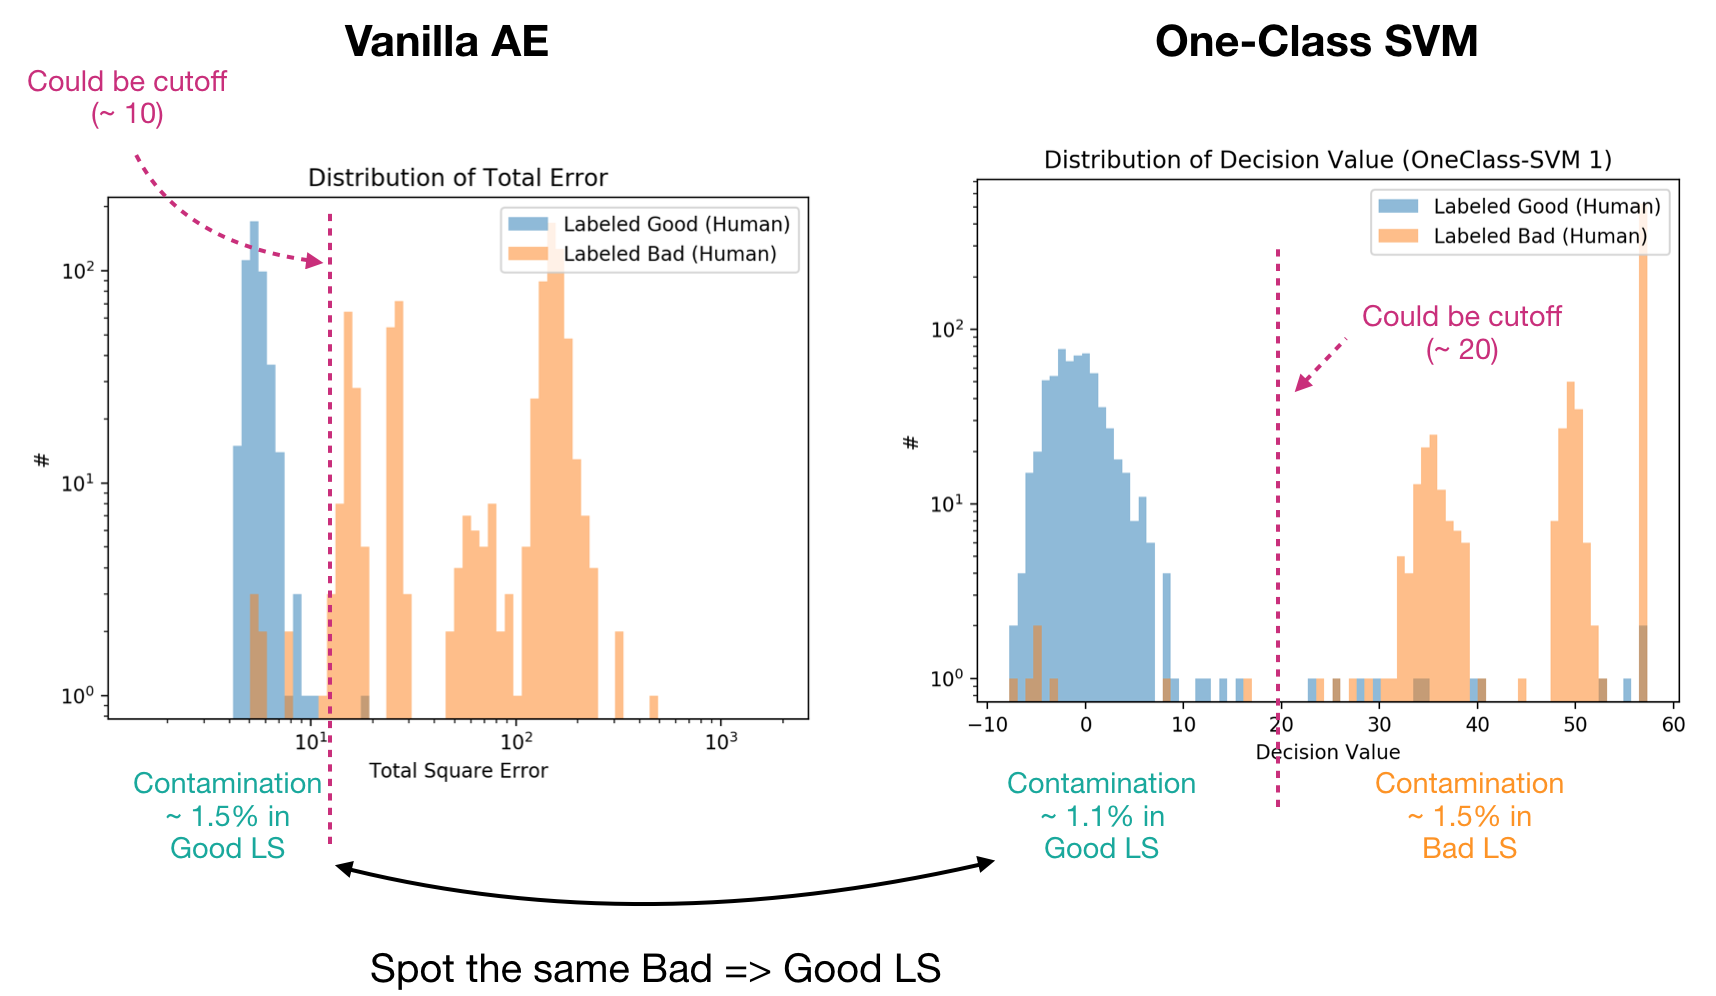
\includegraphics[width=\textwidth]{images/reco/2016/decision_value_dist.png}
    \caption{Distribution of decision value}
    \label{fig:2016_decision_value_dist}
\end{figure}

For Vanilla AE, the contamination of bad LS falling into good LS is around 1\% over the good LS below the cutoff and there are only a few of good LS falling into bad LS which might be ignorable.

For OneClass-SVM, the contamination LS that bad falling into good LS is almost the same as Vanilla AE does. There is no coincidence for a totally different approach of model train and spot the same thing. This might implicitly imply that it either came from some imperfection of data in the training and testing or some kind of malfunction in the sub-system could not propagate into JetHT physics objects.

As can be seen in the distribution, there is no clear grey zone for this study so far.

\subsection{Example of square error from reconstruction}
Figure \ref{fig:2016_example_se} shows the example of LS reconstruction which calculated from $x$ and $\tilde{x}$ between good and bad LS.
\begin{figure}[h!]
    \centering
    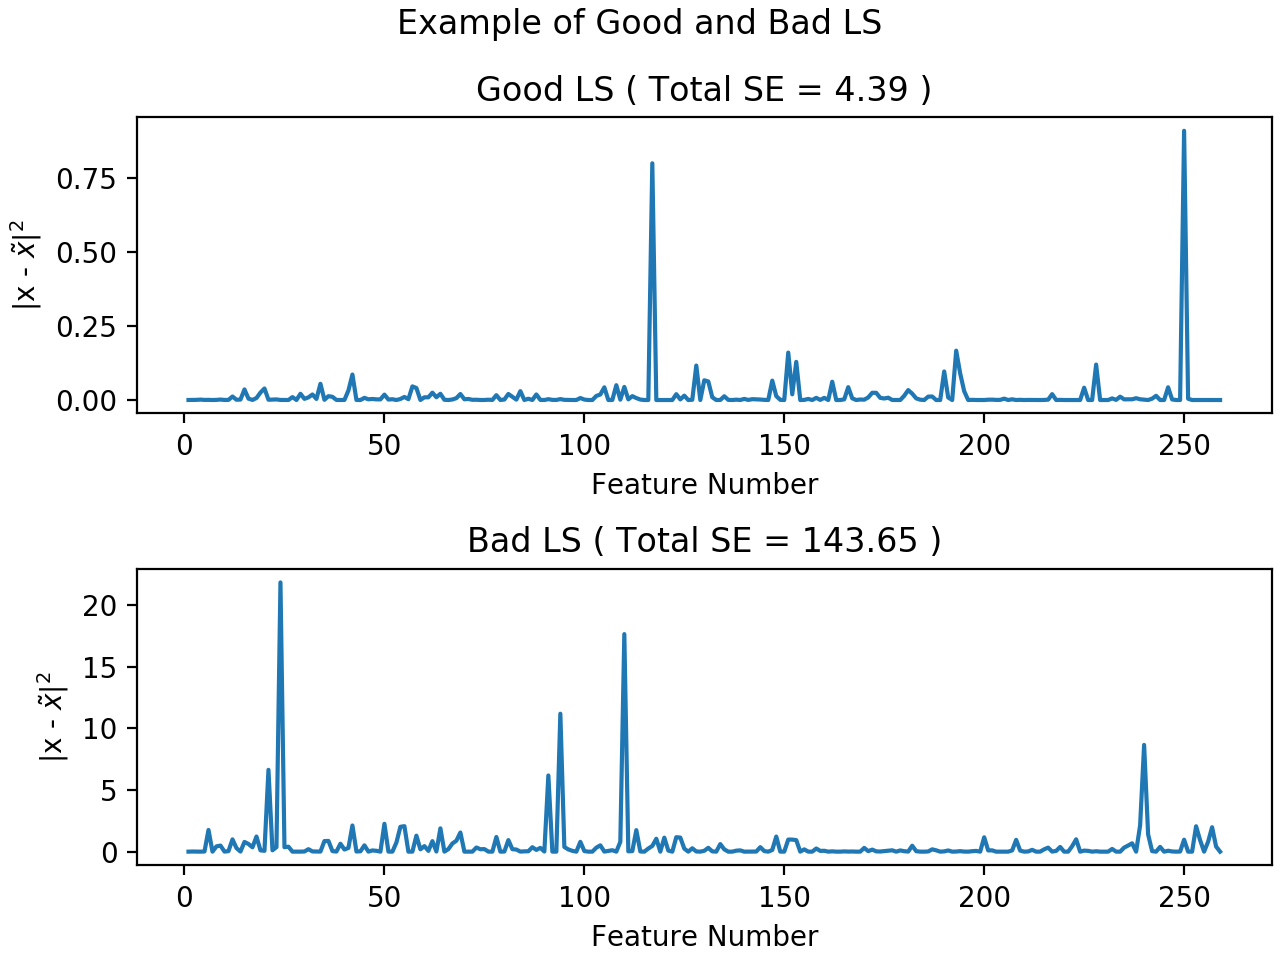
\includegraphics[width=0.8\textwidth]{images/reco/2016/example_se.png}
    \caption{Reconstruction error from Vanilla AE}
    \label{fig:2016_example_se}
\end{figure}

\subsection{Extended Investigation}
It may be questioned why many of bad LS seems to have a group of bad LS as you have seen in the plot of hyperspace and few collections of bad LS in decision value distribution (As the black arrow that links between the distribution and 2D-hyperspace). In this section, I want to explicitly prove that the model really sees that the right cluster is the worse bad LS and closer to tubular is less bad LS which decision value has to be quite similar to good LS. In order to prove that, I choose our best candidate to shade the decision value as z-axis color to represent how bad LS in each data point is as in Figure \ref{fig:2016_guess_visual}. The result strongly agrees that there are obvious bad lumisection and less badness as it gets closer to the green band.
\begin{figure}[h!]
    \centering
    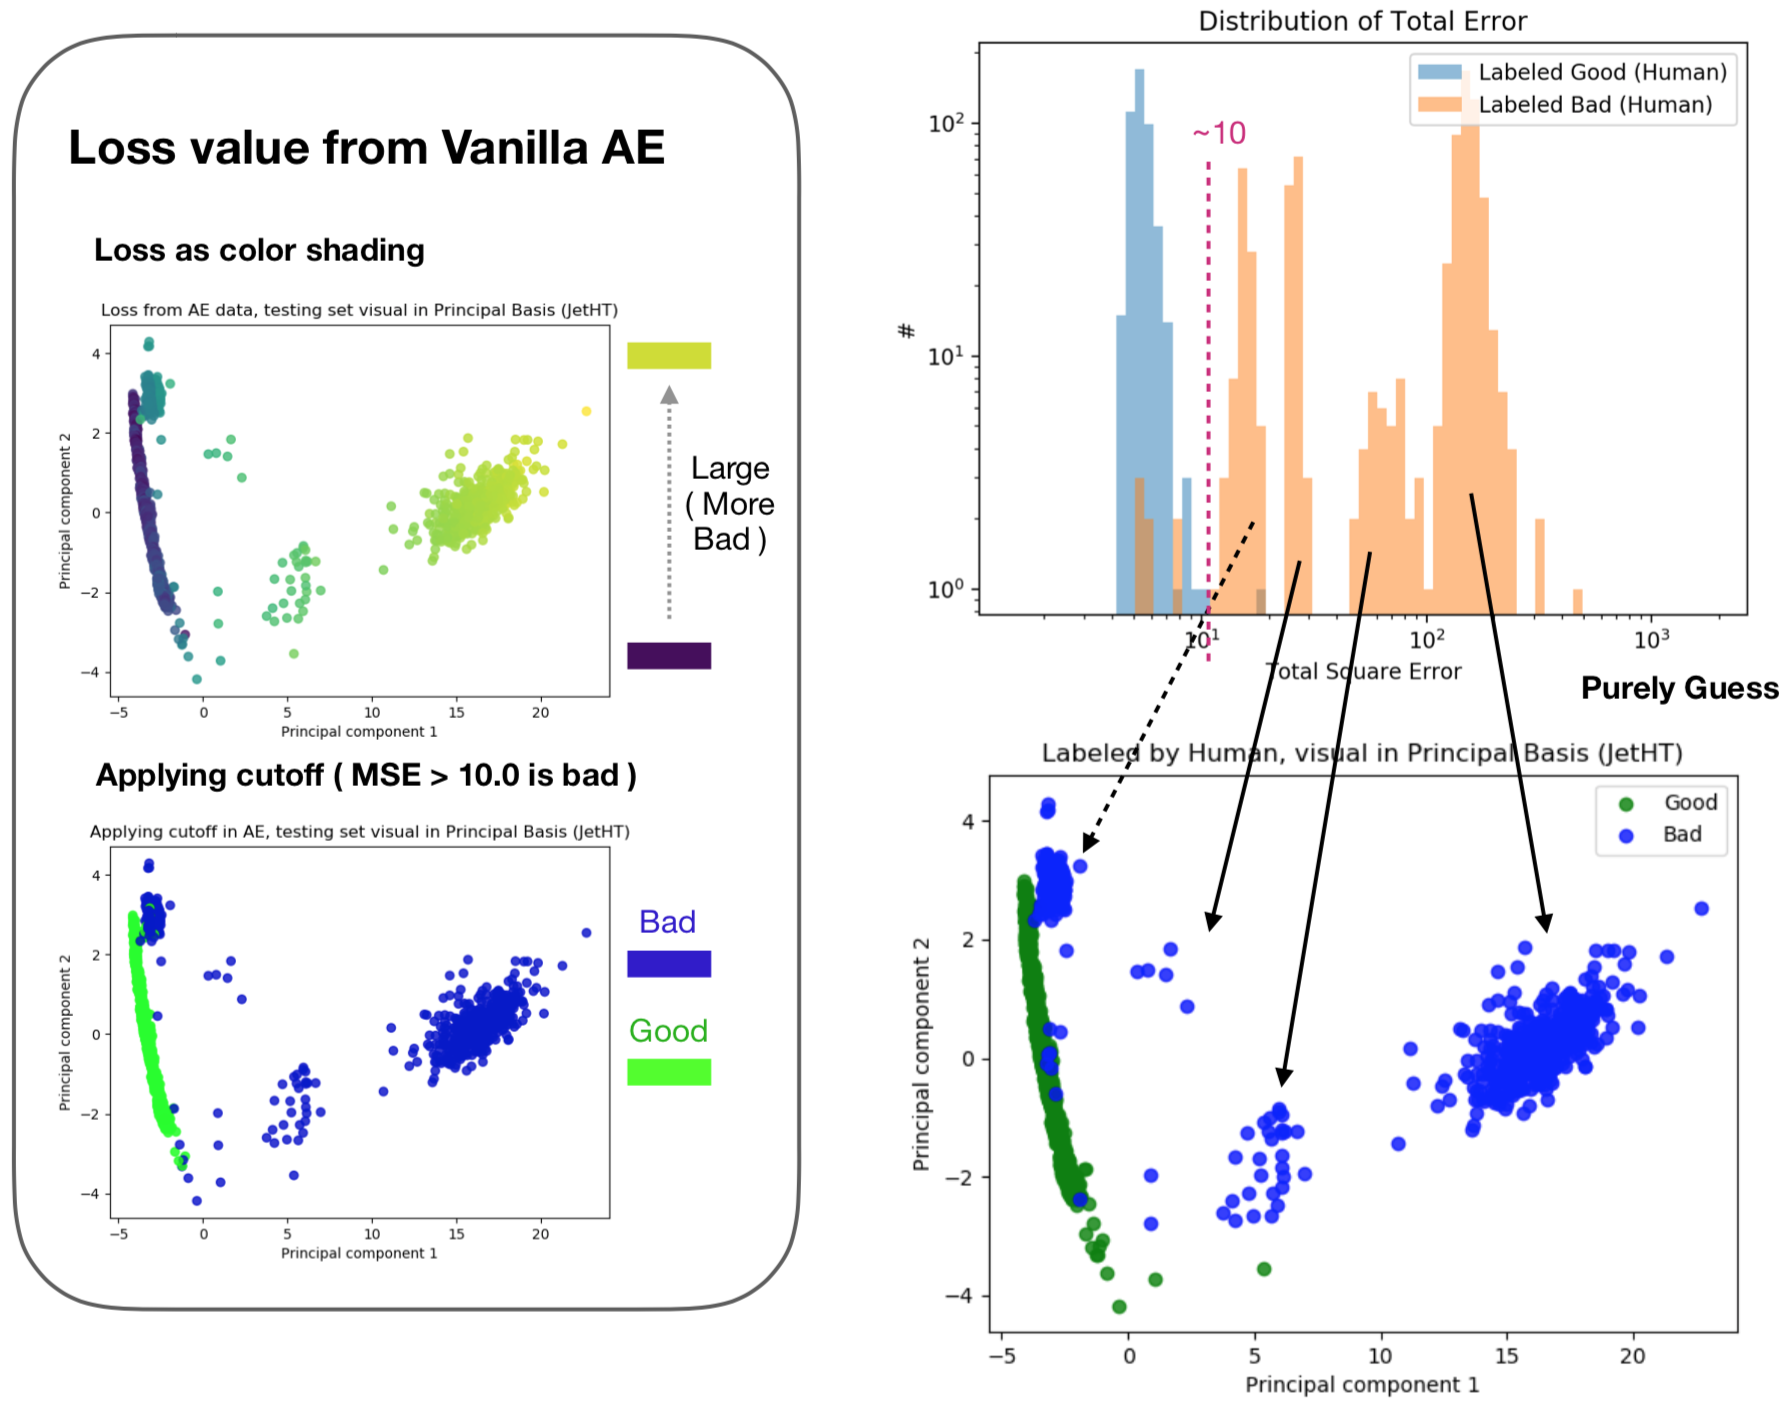
\includegraphics[width=\textwidth]{images/reco/2016/guess_visual.png}
    \caption{Colorize reconstruction error from Vanilla AE}
    \label{fig:2016_guess_visual}
\end{figure}


%%%%%%%%%%%%%%%%%
%     2018
%%%%%%%%%%%%%%%%%

\section{2018 Datasets}

\subsection{Primary Analysis}
For 2018 data, we dig a bit more to understand which cause the badness of bad LS by taking sub-system label into account from RR's API. There is plenty of sub-systems in CMS detector. In order to roughly understand the malfunction of sub-system, we decided to pull label only for HCAL, ECAL, TRACKER and MUON detector which are the main part of the detector.

To roughly describe each feature contribute to each principal component, we extract the element in matrix transform (equivalent to an element in each eigenvector) and take the absolute value to consider only for the magnitude and ignore the direction in the space where it directly proportional to the contribution of each one.
The spectrum of contribution will provide in the following hyperspace of each primary dataset.

\begin{figure}[h!]
\centering
    \begin{subfigure}[b]{0.49\linewidth}
        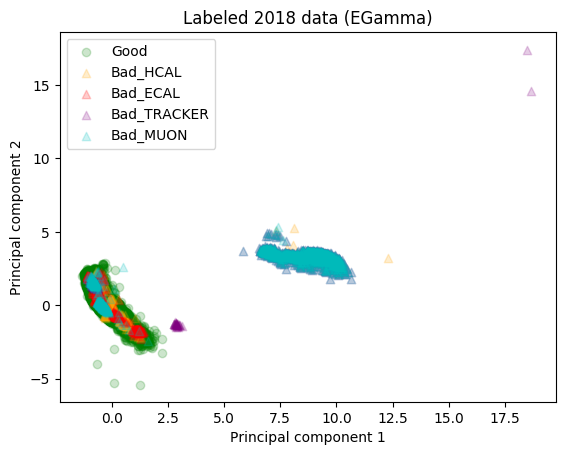
\includegraphics[width=\linewidth]{images/reco/2018/EGamma_subsystem_label.png}
        \caption{Full range}
    \end{subfigure}
    \begin{subfigure}[b]{0.49\linewidth}
        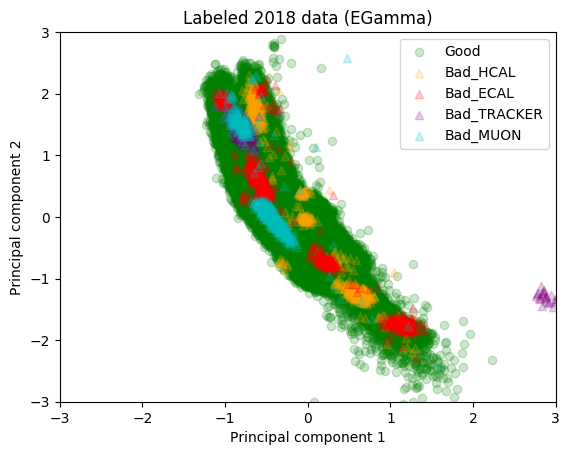
\includegraphics[width=\linewidth]{images/reco/2018/EGamma_subsystem_label_short_range.png}
        \caption{Zoom in}
    \end{subfigure}
    \begin{subfigure}[b]{0.49\linewidth}
        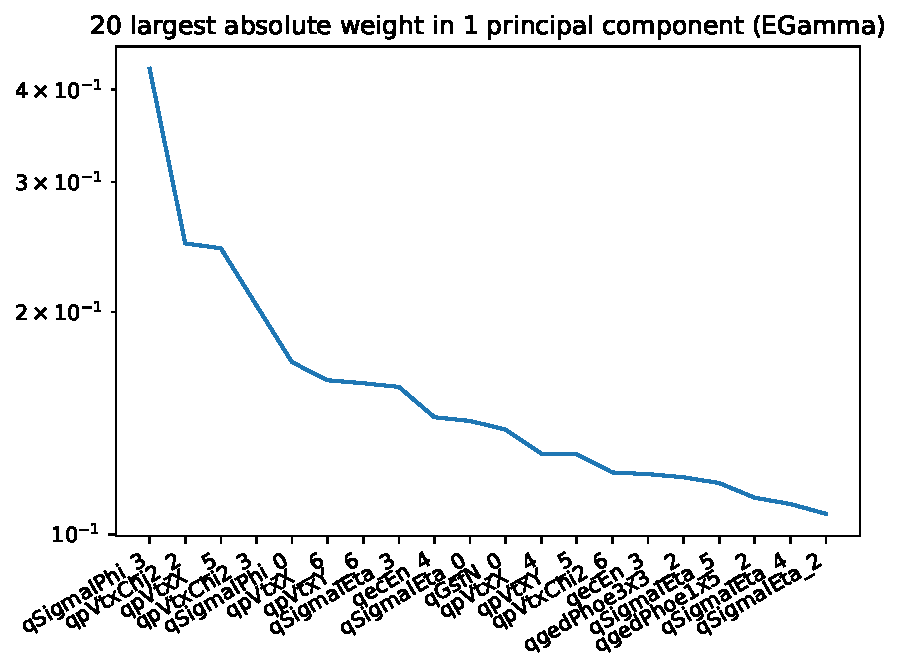
\includegraphics[width=\linewidth]{images/reco/2018/feature_2/EGamma_pc1.pdf}
        \caption{Contribution of features on PC1 \\ (explained variance ratio = 0.31)}
    \end{subfigure}
    \begin{subfigure}[b]{0.49\linewidth}
        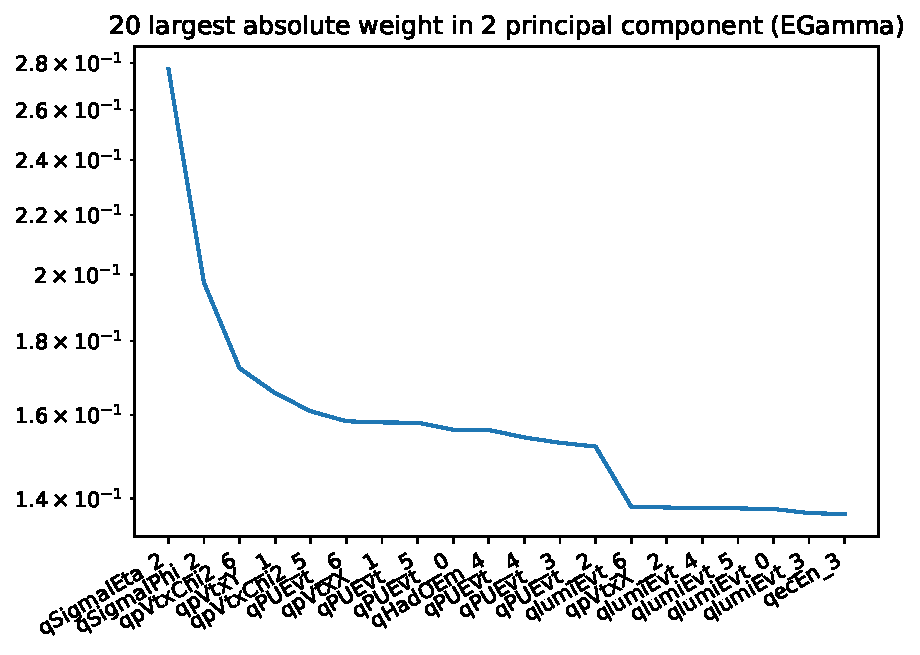
\includegraphics[width=\linewidth]{images/reco/2018/feature_2/EGamma_pc2.pdf}
        \caption{Contribution of features on PC2 \\ (explained variance ratio = 0.25)}
    \end{subfigure}
\caption{Two principal components of EGamma}
\label{fig:2018_EGamma_subsystem_label}
\end{figure}

\begin{figure}[h!]
\centering
    \begin{subfigure}[b]{0.49\linewidth}
        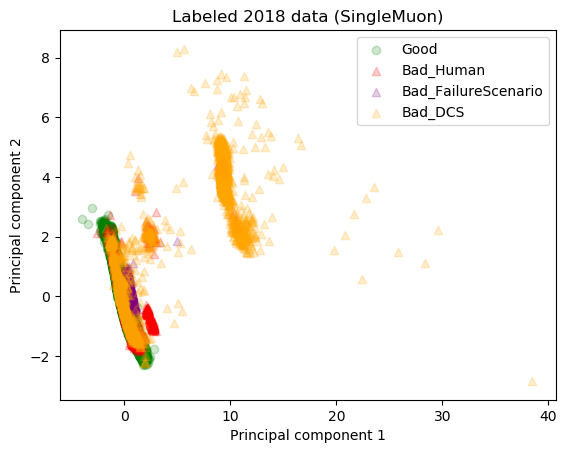
\includegraphics[width=\linewidth]{images/reco/2018/SingleMuon_label_separate.png}
        \caption{Full range}
    \end{subfigure}
    \begin{subfigure}[b]{0.49\linewidth}
        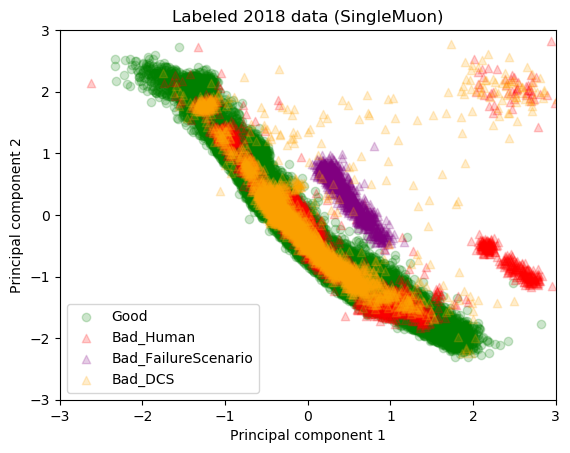
\includegraphics[width=\linewidth]{images/reco/2018/SingleMuon_label_separate_short_range.png}
        \caption{Zoom in}
    \end{subfigure}
    \begin{subfigure}[b]{0.49\linewidth}
        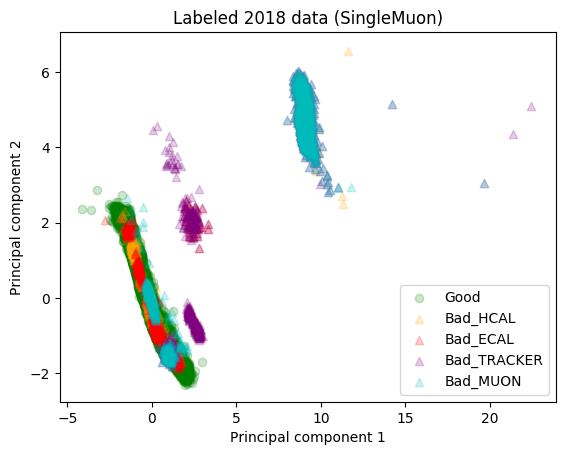
\includegraphics[width=\linewidth]{images/reco/2018/SingleMuon_subsystem_label.png}
        \caption{Full range}
    \end{subfigure}
    \begin{subfigure}[b]{0.49\linewidth}
        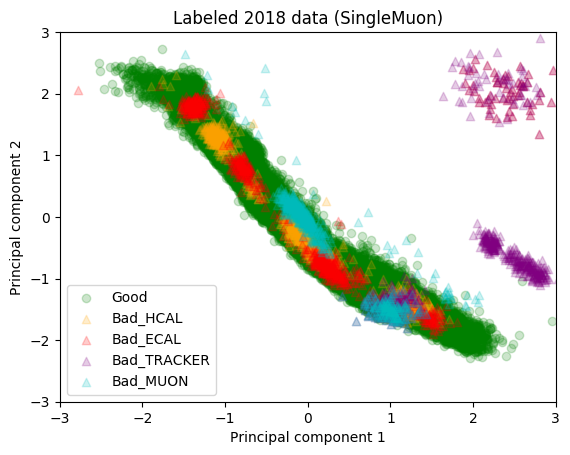
\includegraphics[width=\linewidth]{images/reco/2018/SingleMuon_subsystem_label_short_range.png}
        \caption{Zoom in}
    \end{subfigure}
    \begin{subfigure}[b]{0.49\linewidth}
        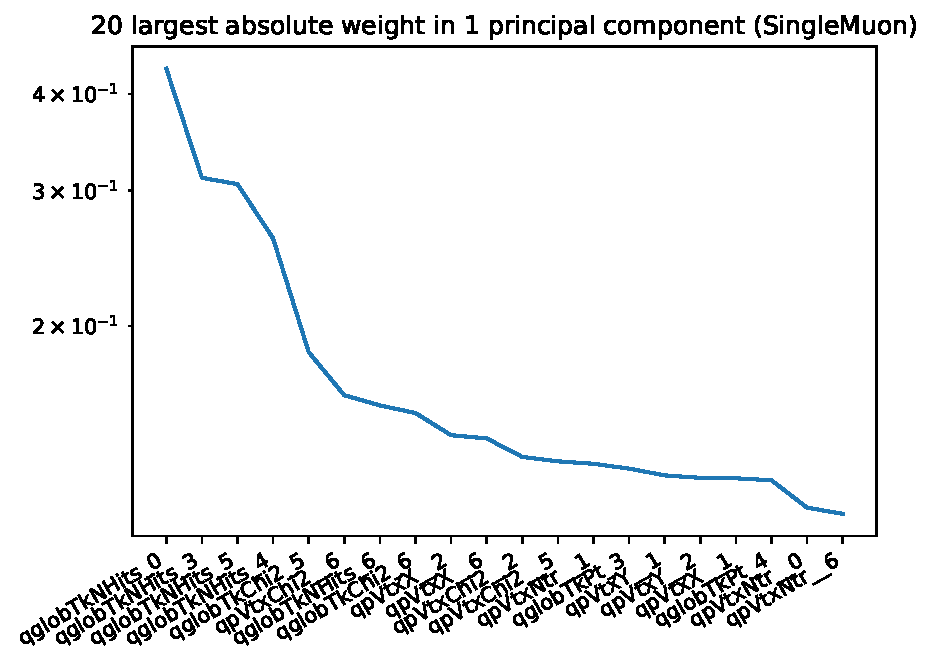
\includegraphics[width=\linewidth]{images/reco/2018/feature_2/SingleMuon_pc1.pdf}
        \caption{Contribution of features on PC1 \\ (explained variance ratio = 0.37)}
    \end{subfigure}
    \begin{subfigure}[b]{0.49\linewidth}
        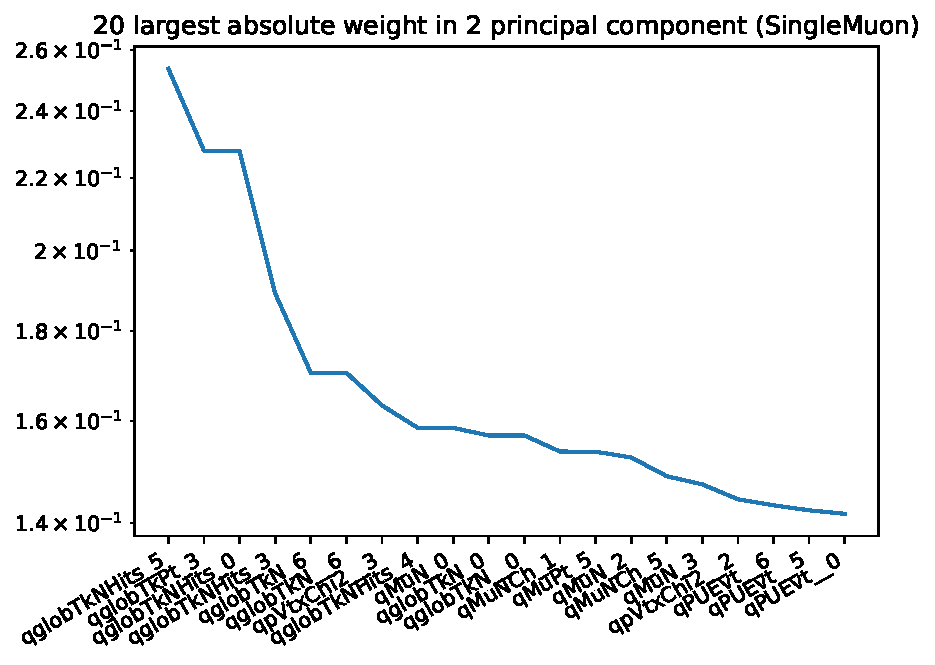
\includegraphics[width=\linewidth]{images/reco/2018/feature_2/SingleMuon_pc2.pdf}
        \caption{Contribution of features on PC2 \\ (explained variance ratio = 0.22)}
    \end{subfigure}
    \caption{Two principal components of Single Muon}
\label{fig:2018_SingleMuon_subsystem_label}
\end{figure}


\begin{figure}[h!]
\centering
    \begin{subfigure}[b]{0.49\linewidth}
        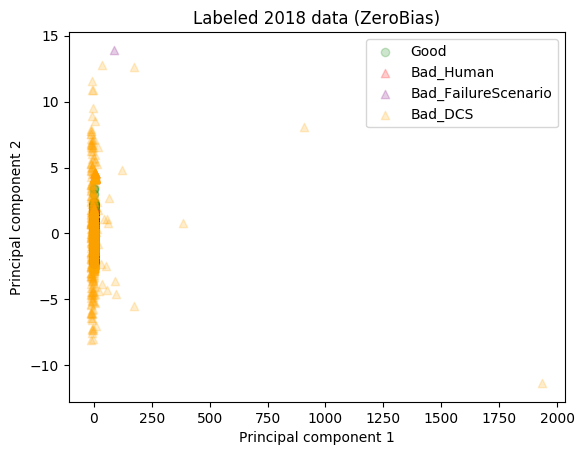
\includegraphics[width=\linewidth]{images/reco/2018/ZeroBias_label_separate.png}
        \caption{Full range}
    \end{subfigure}
    \begin{subfigure}[b]{0.49\linewidth}
        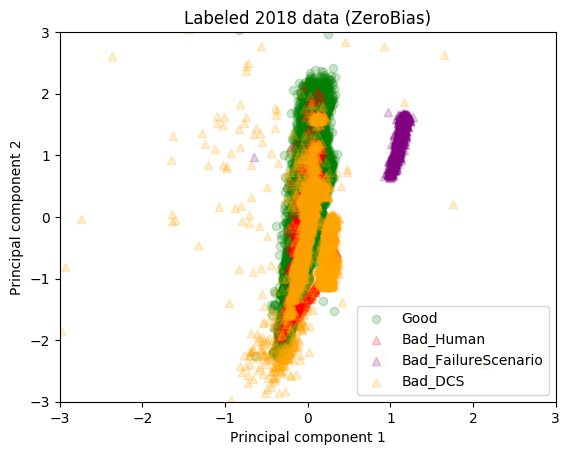
\includegraphics[width=\linewidth]{images/reco/2018/ZeroBias_label_separate_short_range.png}
        \caption{Zoom in}
    \end{subfigure}
    \begin{subfigure}[b]{0.49\linewidth}
        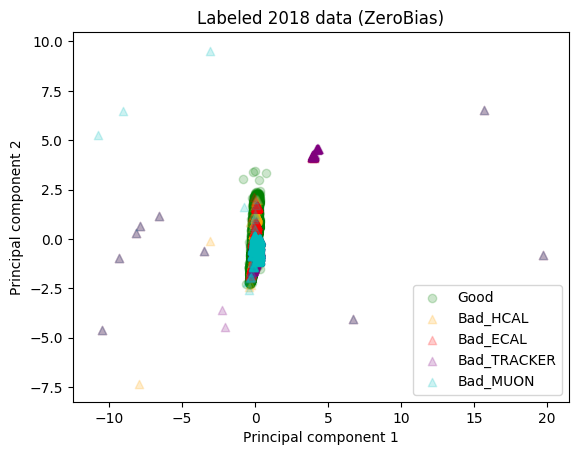
\includegraphics[width=\linewidth]{images/reco/2018/ZeroBias_subsystem_label.png}
        \caption{Full range}
    \end{subfigure}
    \begin{subfigure}[b]{0.49\linewidth}
        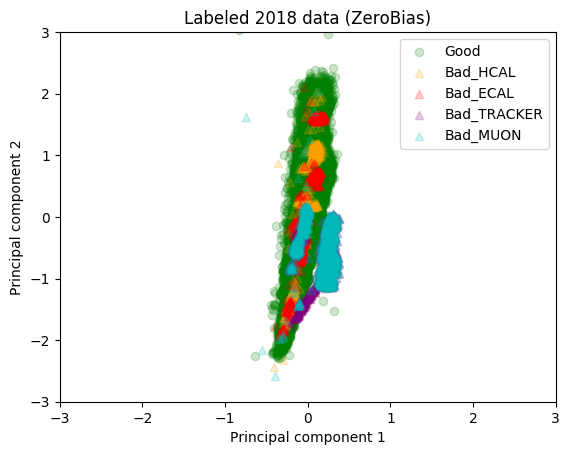
\includegraphics[width=\linewidth]{images/reco/2018/ZeroBias_subsystem_label_short_range.png}
        \caption{Zoom in}
    \end{subfigure}
    \begin{subfigure}[b]{0.49\linewidth}
        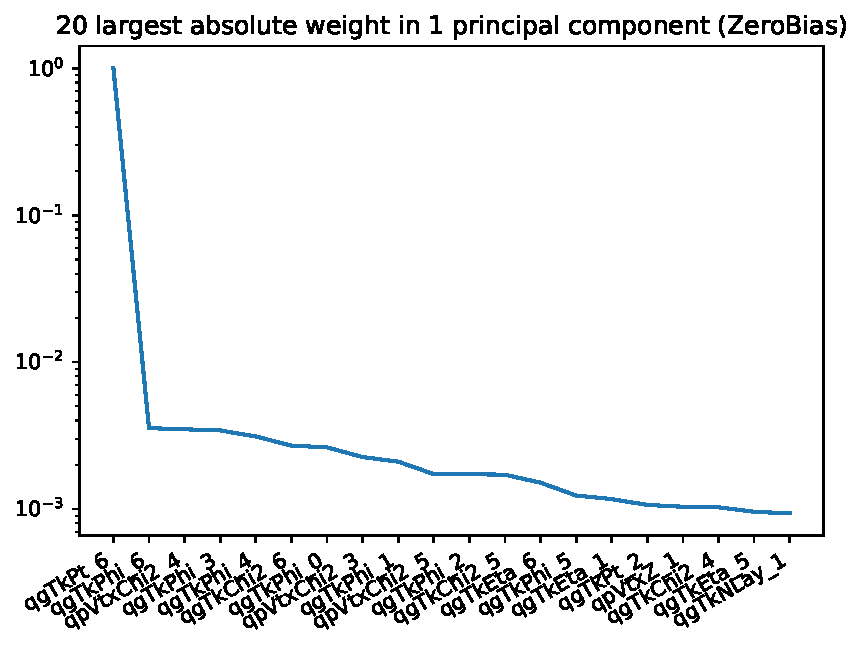
\includegraphics[width=\linewidth]{images/reco/2018/feature_2/ZeroBias_pc1.pdf}
        \caption{Contribution of features on PC1 \\ (explained variance ratio = 0.89)}
    \end{subfigure}
    \begin{subfigure}[b]{0.49\linewidth}
        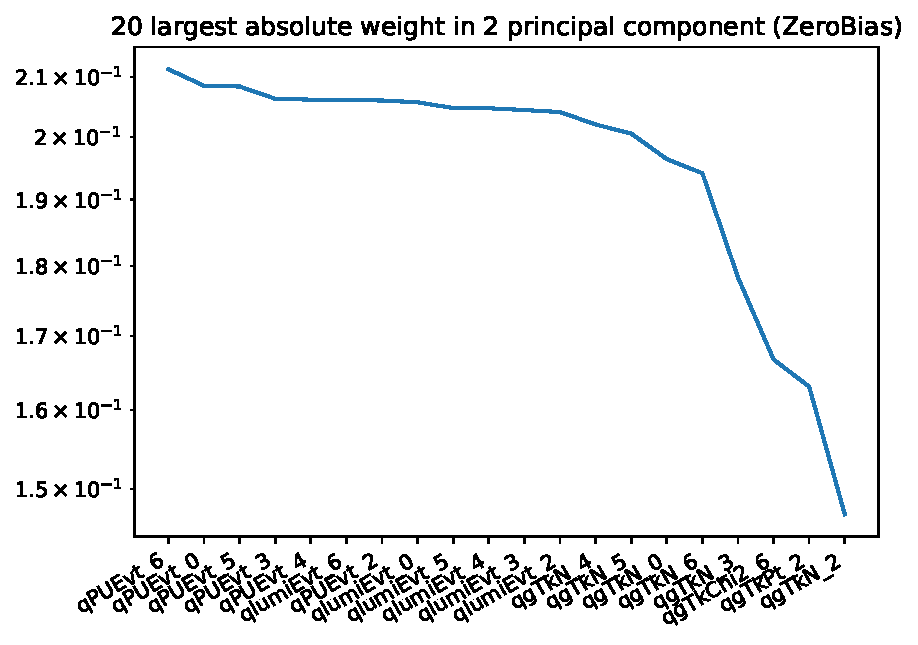
\includegraphics[width=\linewidth]{images/reco/2018/feature_2/ZeroBias_pc2.pdf}
        \caption{Contribution of features on PC2 \\ (explained variance ratio = 0.0225)}
    \end{subfigure}
    \caption{Two principal components of ZeroBias}
\label{fig:2018_ZeroBias_subsystem_label}
\end{figure}

\begin{figure}[h!]
\centering
    \begin{subfigure}[b]{0.49\linewidth}
        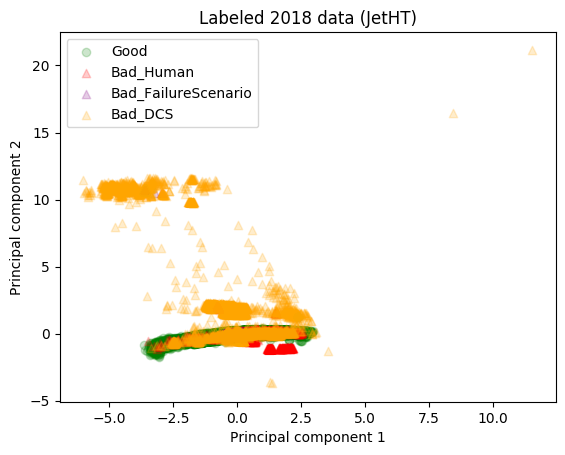
\includegraphics[width=\linewidth]{images/reco/2018/JetHT_label_separate.png}
        \caption{Full range}
    \end{subfigure}
    \begin{subfigure}[b]{0.49\linewidth}
        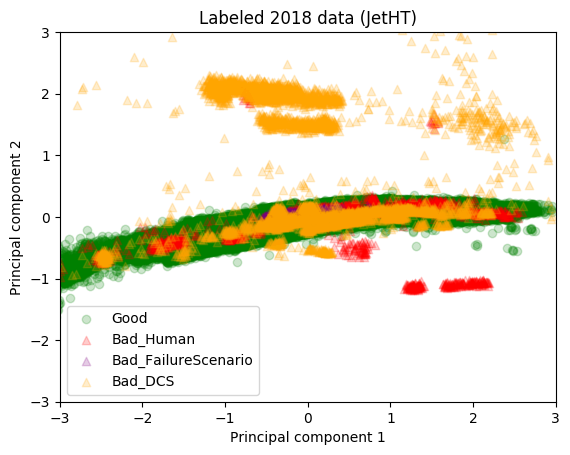
\includegraphics[width=\linewidth]{images/reco/2018/JetHT_label_separate_short_range.png}
        \caption{Zoom in}
    \end{subfigure}
    \begin{subfigure}[b]{0.49\linewidth}
        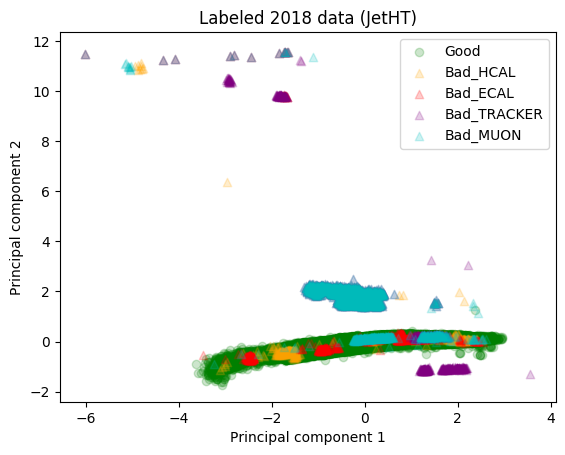
\includegraphics[width=\linewidth]{images/reco/2018/JetHT_subsystem_label.png}
        \caption{Full range}
    \end{subfigure}
    \begin{subfigure}[b]{0.49\linewidth}
        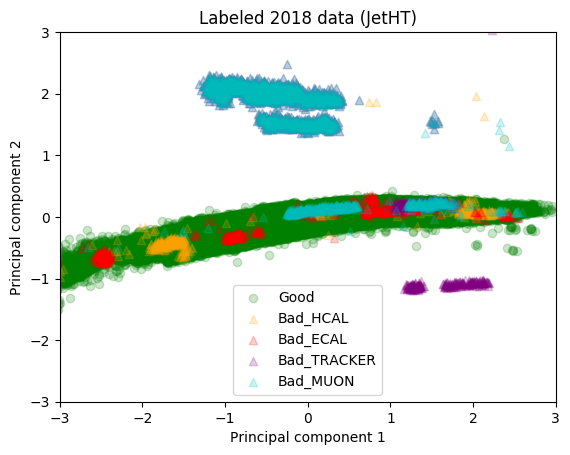
\includegraphics[width=\linewidth]{images/reco/2018/JetHT_subsystem_label_short_range.png}
        \caption{Zoom in}
    \end{subfigure}
    \begin{subfigure}[b]{0.49\linewidth}
        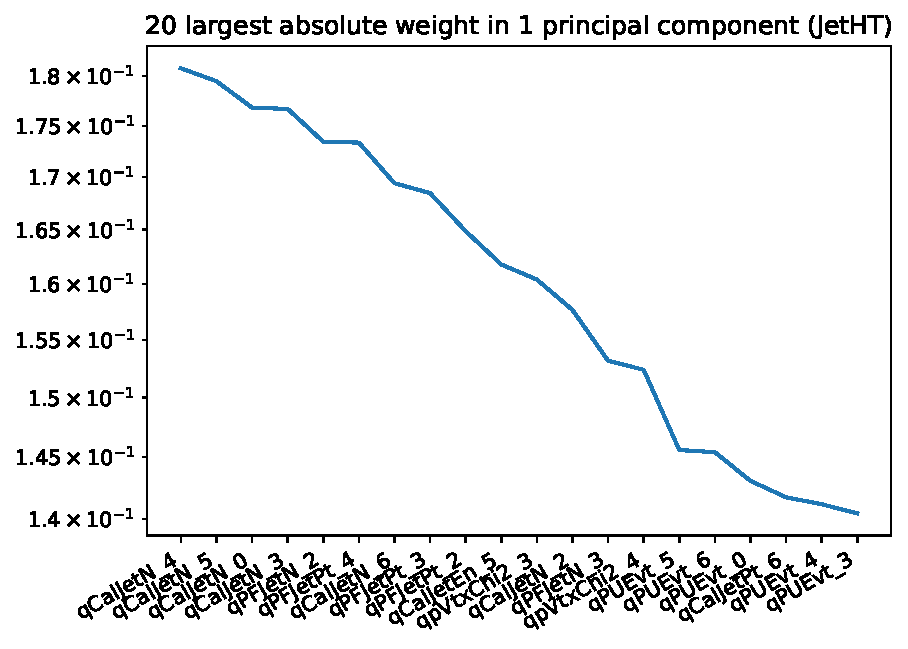
\includegraphics[width=\linewidth]{images/reco/2018/feature_2/JetHT_pc1.pdf}
        \caption{Contribution of features on PC1 \\ (explained variance ratio = 0.45)}
    \end{subfigure}
    \begin{subfigure}[b]{0.49\linewidth}
        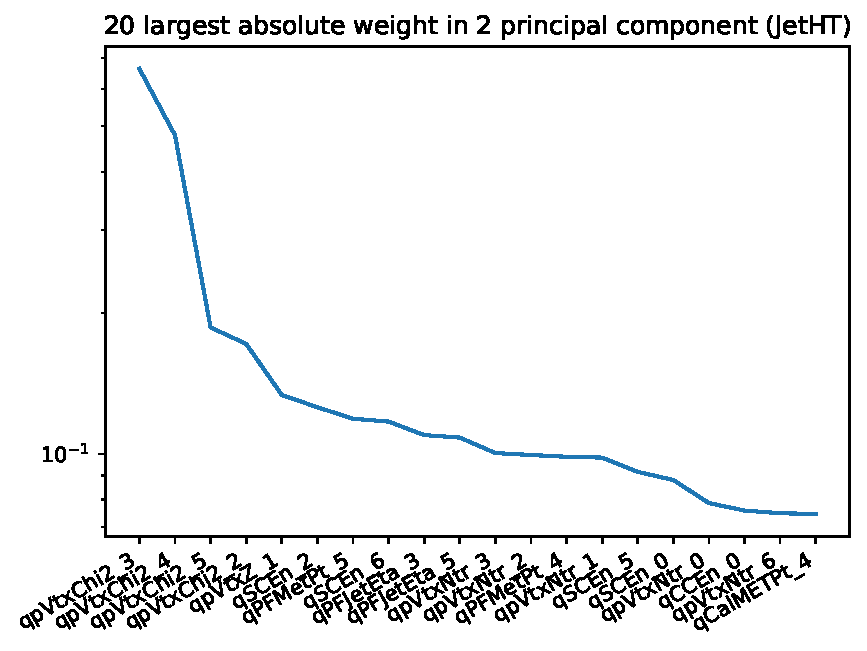
\includegraphics[width=\linewidth]{images/reco/2018/feature_2/JetHT_pc2.pdf}
        \caption{Contribution of features on PC2 \\ (explained variance ratio = 0.21)}
    \end{subfigure}
    \caption{Two principal components of JetHT}
\label{fig:2018_JetHT_subsystem_label}
\end{figure}

According to Figure (\ref{fig:2018_EGamma_subsystem_label}, \ref{fig:2018_SingleMuon_subsystem_label}, \ref{fig:2018_ZeroBias_subsystem_label}, \ref{fig:2018_JetHT_subsystem_label}), It's obviously to tell that the cluster of outlier are mainly consists of malfunction from MUON and TRACKER sub-detector. Not only the outlier that has an interesting pattern but clustering in inlier is also remarkably considerable as clustering mainly from a malfunction of ECAL and HCAL that located near or inside the green band.

Please note that the calculation of the matrix transform exclude failure scenario since it's a fake data and it might leading to a weird correlation in covariance matrix.
The following list is the list of important features that highly correlated to the rest of them in our dataset
\begin{itemize}
    \item From Figure \ref{fig:2018_EGamma_subsystem_label}, qpVt in transverse direction and qSigmalEta contribute in first component.
    Secondly, second component mostly consists of qPUEvt and qlumiEvt. Lastly, there are overlapping feature where both of them sharing the different value which are qSigmalPhi and qpVtxChi2.
    \item Regarding Figure \ref{fig:2018_SingleMuon_subsystem_label}, qglobTkChi2 and qpVtx in perpendicular direction of the beam are dominated in first component and second component mostly consists of qPUEvt, qMuN and qMuNCh orderly.
    The only overlapping feature in SingleMuon is qglobTkNHits.
    \item For ZeroBias in Figure \ref{fig:2018_ZeroBias_subsystem_label}, both qgTkPt and qgTkPhi highly dominate in first component.
    Second component has smaller correlation which the faetures are qPUEvt, qlumiEvt and qgTkN.
    \item First component are constantly diminated to qCalJetN, qCalJetPt and qPUEvt orderly according to Figure \ref{fig:2018_JetHT_subsystem_label}.
    Feature qpVtxChi2, qPFMetPt and qPFJetEta also fairly equally contribute to the second component. 
\end{itemize}

\subsection{Performance}
\subsubsection{1) Include low statistics (fill null with zero) and testing with only bad LS form human}
Train with feature set 1 and the result has shown in Figure \ref{fig:2018_f1_ae_performance}.

The performance of AE for EGamma primary dataset is totally inefficient and even worse than randomly picking up which means that the model even saw most of bad LS even looks better than many good LS in the testing datasets. The rest of them is fairly acceptable but still not enough to exploit in the real system. Another interesting spot is the performance between a couple of AE in SingleMuon PD. 

\begin{figure}[h!]
\centering
    \begin{subfigure}[b]{0.49\linewidth}
        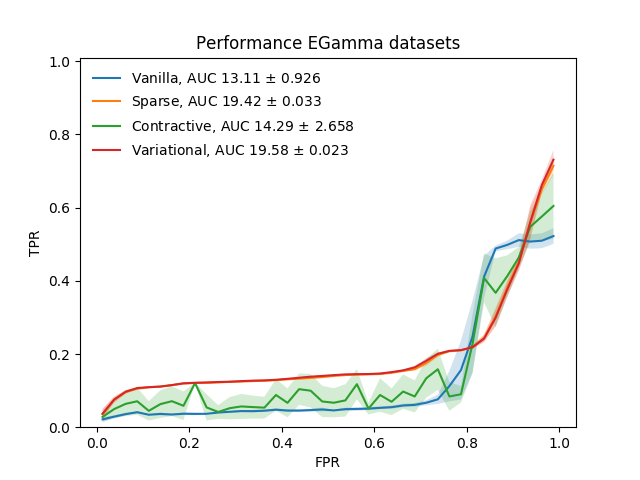
\includegraphics[width=\linewidth]{images/reco/2018/feature_1/performance_EGamma_VanillaSparseContractiveVariational.png}
        \caption{EGamma}
    \end{subfigure}
    \begin{subfigure}[b]{0.49\linewidth}
        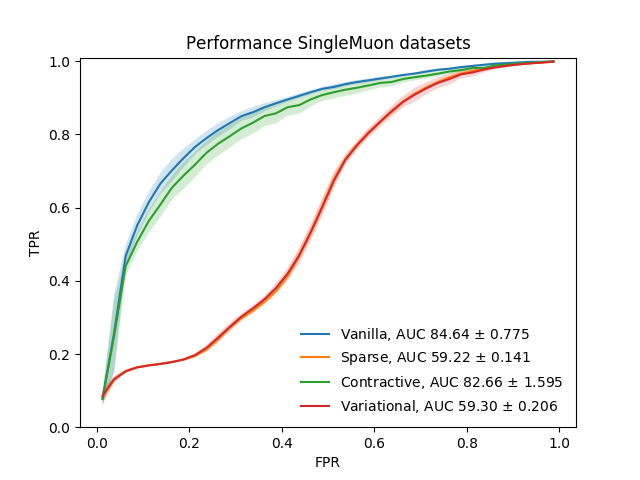
\includegraphics[width=\linewidth]{images/reco/2018/feature_1/performance_SingleMuon_VanillaSparseContractiveVariational.png}
        \caption{SingleMuon}
    \end{subfigure}
    \begin{subfigure}[b]{0.49\linewidth}
        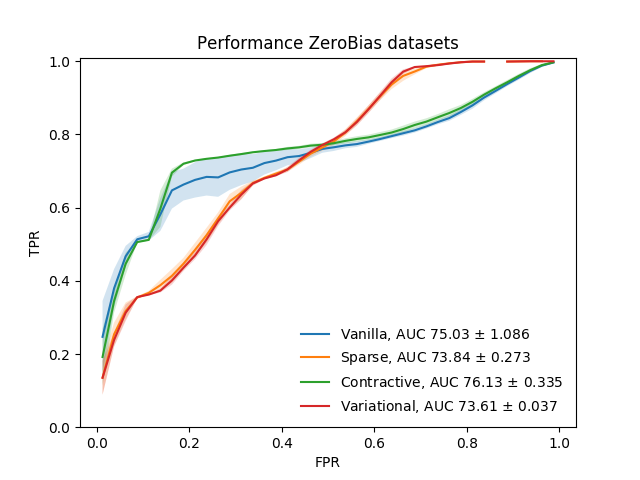
\includegraphics[width=\linewidth]{images/reco/2018/feature_1/performance_ZeroBias_VanillaSparseContractiveVariational.png}
        \caption{ZeroBias}
    \end{subfigure}
    \begin{subfigure}[b]{0.49\linewidth}
        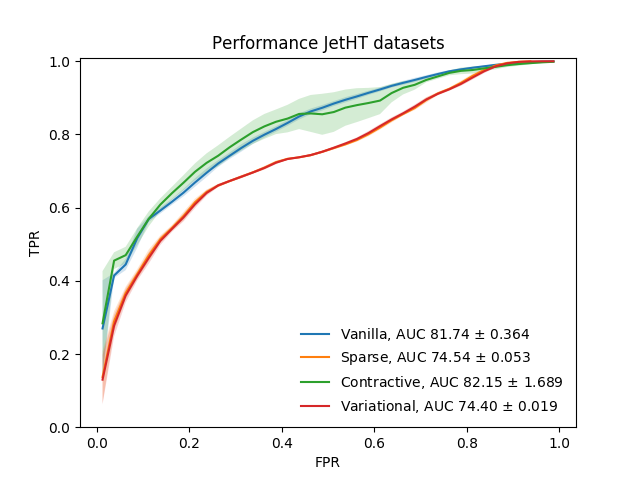
\includegraphics[width=\linewidth]{images/reco/2018/feature_1/performance_JetHT_VanillaSparseContractiveVariational.png}
        \caption{JetHT}
    \end{subfigure}
    \caption{Model performance for feature set 1 with 2018 data}
\label{fig:2018_f1_ae_performance}
\end{figure}

Figure \ref{fig:2018_f1_exteded_ae_performance} has demonstrated that even extended model has been combined various constraints that we know but it still not improves any further in terms of performance. Nevertheless, it has remarkable stability, especially for ContractiveVariational AE.

\begin{figure}[h!]
\centering
    \begin{subfigure}[b]{0.49\linewidth}
        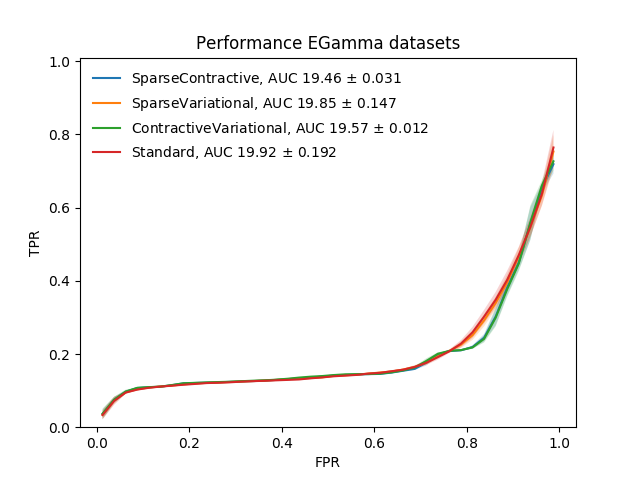
\includegraphics[width=\linewidth]{images/reco/2018/feature_1/performance_EGamma_SparseContractiveSparseVariationalContractiveVariationalStandard.png}
        \caption{EGamma}
    \end{subfigure}
    \begin{subfigure}[b]{0.49\linewidth}
        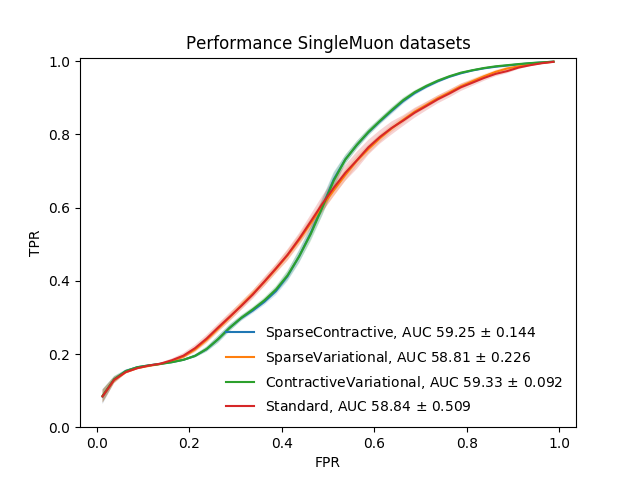
\includegraphics[width=\linewidth]{images/reco/2018/feature_1/performance_SingleMuon_SparseContractiveSparseVariationalContractiveVariationalStandard.png}
        \caption{SingleMuon}
    \end{subfigure}
    \begin{subfigure}[b]{0.49\linewidth}
        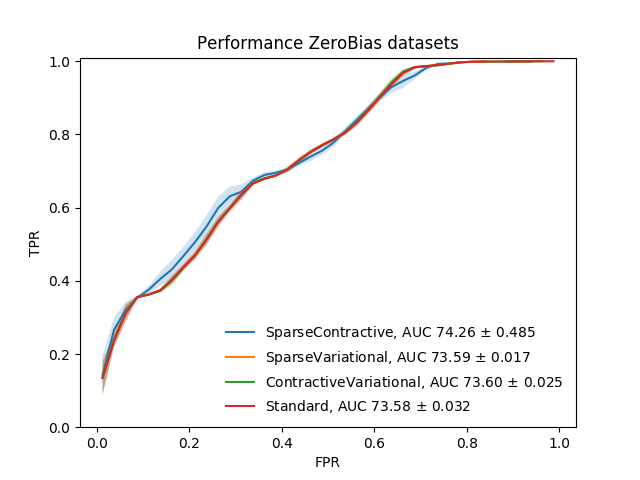
\includegraphics[width=\linewidth]{images/reco/2018/feature_1/performance_ZeroBias_SparseContractiveSparseVariationalContractiveVariationalStandard.png}
        \caption{ZeroBias}
    \end{subfigure}
    \begin{subfigure}[b]{0.49\linewidth}
        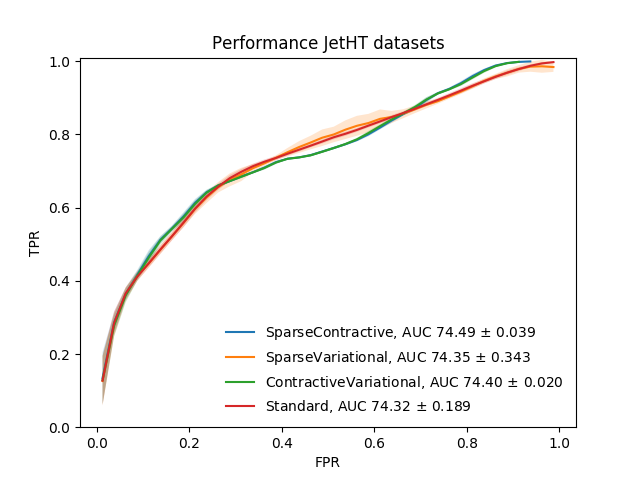
\includegraphics[width=\linewidth]{images/reco/2018/feature_1/performance_JetHT_SparseContractiveSparseVariationalContractiveVariationalStandard.png}
        \caption{JetHT}
    \end{subfigure}
    \caption{Extended model performance for feature set 1 with 2018 data}
\label{fig:2018_f1_exteded_ae_performance}
\end{figure}


\subsubsection{2) Exclude low statistics (Filter LS that has low EventsPerLs with value in the settings)}
Train with feature set 1 and the result has shown in Figure \ref{fig:2018_f2_ae_performance}.
We also perform an extended autoencoder for testing with this case, Figure \ref{fig:2018_f2_extended_ae_performance} has shown the stability and smoothness of the threshold as we have seen in Figure \ref{fig:2018_f1_exteded_ae_performance}.

\begin{figure}[h!]
\centering
    \begin{subfigure}[b]{0.49\linewidth}
        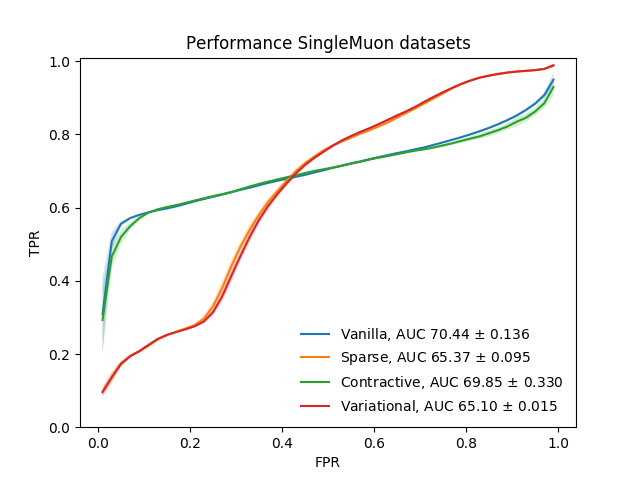
\includegraphics[width=\linewidth]{images/reco/2018/feature_2/performance_SingleMuon_VanillaSparseContractiveVariational.png}
        \caption{Full range}
    \end{subfigure}
    \begin{subfigure}[b]{0.49\linewidth}
        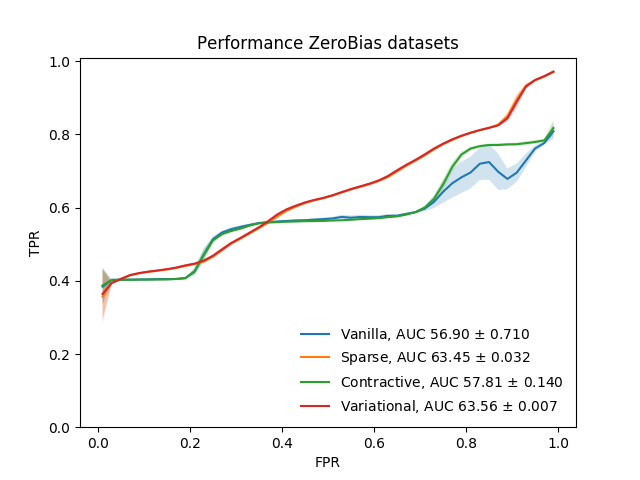
\includegraphics[width=\linewidth]{images/reco/2018/feature_2/performance_ZeroBias_VanillaSparseContractiveVariational.png}
        \caption{Zoom in}
    \end{subfigure}
    \begin{subfigure}[b]{0.49\linewidth}
        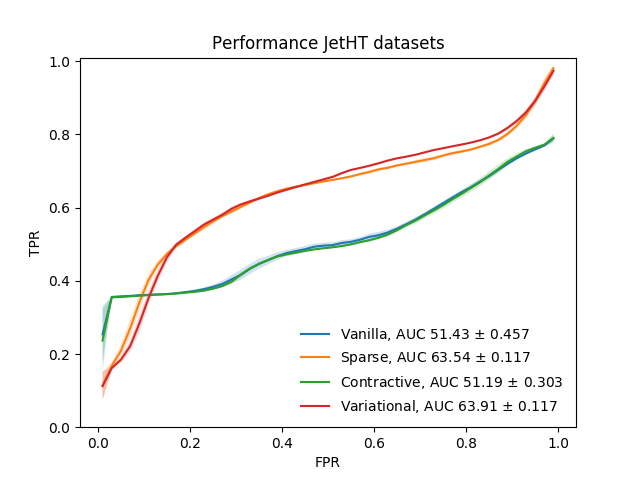
\includegraphics[width=\linewidth]{images/reco/2018/feature_2/performance_JetHT_VanillaSparseContractiveVariational.png}
        \caption{Full range}
    \end{subfigure}
    % \begin{subfigure}[b]{0.49\linewidth}
    %     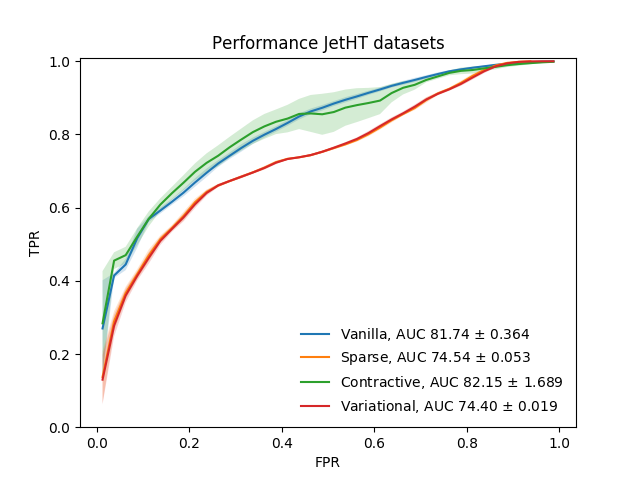
\includegraphics[width=\linewidth]{images/reco/2018/feature_1/performance_JetHT_VanillaSparseContractiveVariational.png}
    %     \caption{Zoom in}
    % \end{subfigure}
    \caption{Model performance for feature set 2 with 2018 data}
\label{fig:2018_f2_ae_performance}
\end{figure}

\begin{figure}[h!]
\centering
    \begin{subfigure}[b]{0.49\linewidth}
        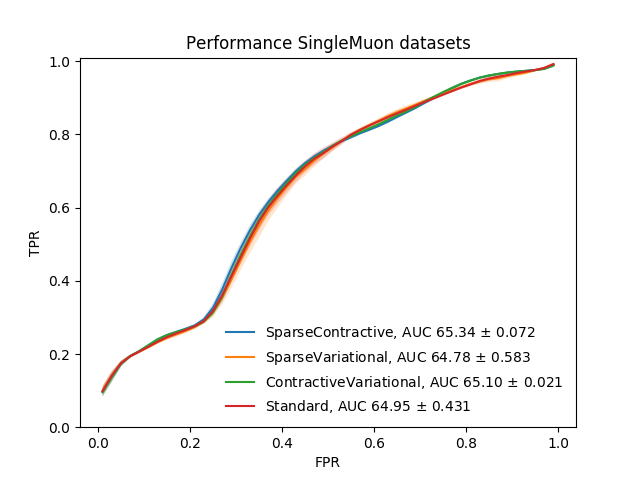
\includegraphics[width=\linewidth]{images/reco/2018/feature_2/performance_SingleMuon_SparseContractiveSparseVariationalContractiveVariationalStandard.png}
        \caption{Full range}
    \end{subfigure}
    \begin{subfigure}[b]{0.49\linewidth}
        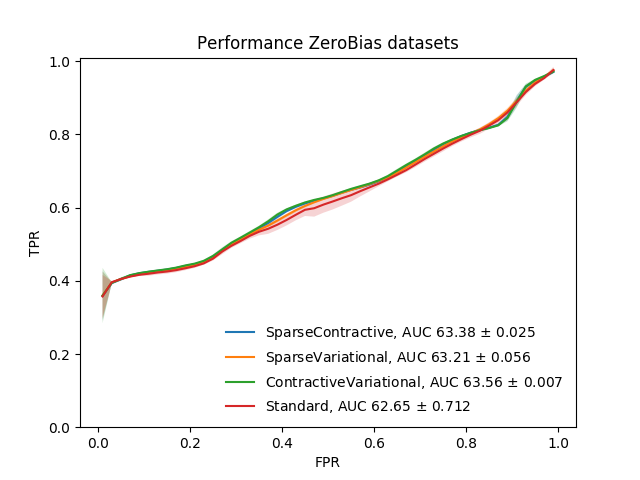
\includegraphics[width=\linewidth]{images/reco/2018/feature_2/performance_ZeroBias_SparseContractiveSparseVariationalContractiveVariationalStandard.png}
        \caption{Zoom in}
    \end{subfigure}
    \begin{subfigure}[b]{0.49\linewidth}
        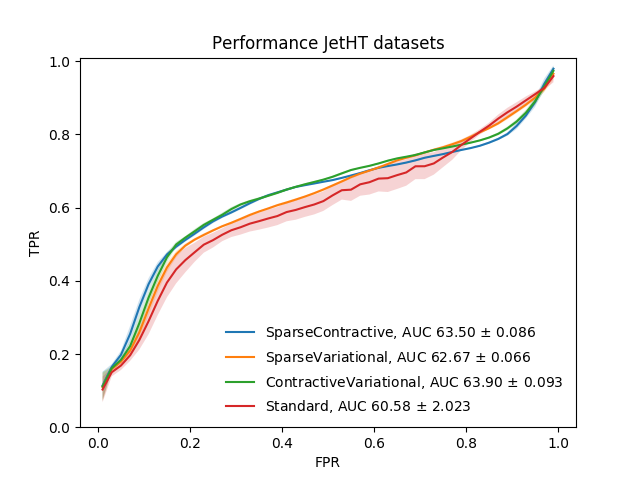
\includegraphics[width=\linewidth]{images/reco/2018/feature_2/performance_JetHT_SparseContractiveSparseVariationalContractiveVariationalStandard.png}
        \caption{Full range}
    \end{subfigure}
    % \begin{subfigure}[b]{0.49\linewidth}
    %     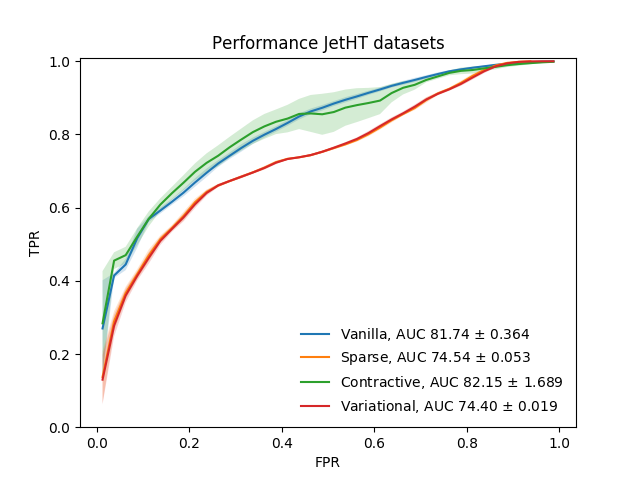
\includegraphics[width=\linewidth]{images/reco/2018/feature_1/performance_JetHT_VanillaSparseContractiveVariational.png}
    %     \caption{Zoom in}
    % \end{subfigure}
    \caption{Extended model performance for feature set 2 with 2018 data}
\label{fig:2018_f2_extended_ae_performance}
\end{figure}

\subsubsection{Distribution of decision value (to find the threshold)}
The distribution of decision value could be seen in Figure \ref{fig:2018_f2_se_dist}

\begin{figure}[h!]
\centering
    \begin{subfigure}[b]{0.49\linewidth}
        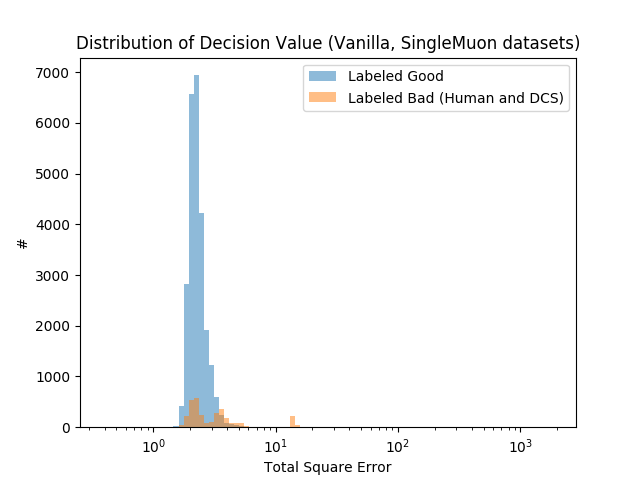
\includegraphics[width=\linewidth]{images/reco/2018/feature_2/se_dist_Vanilla1f2_SingleMuon_unlog.png}
        \caption{SingleMuon}
    \end{subfigure}
    \begin{subfigure}[b]{0.49\linewidth}
        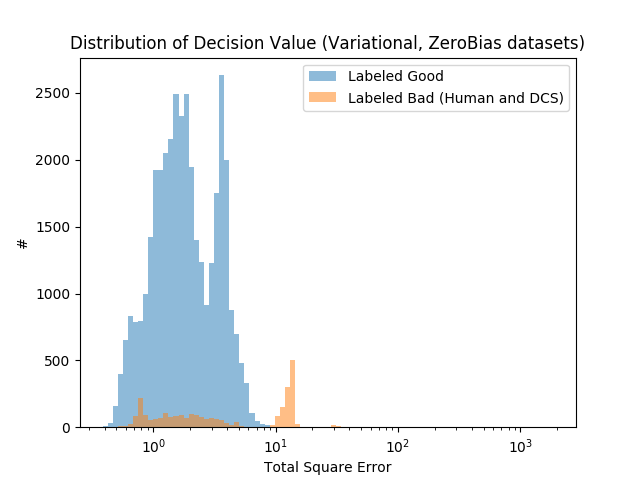
\includegraphics[width=\linewidth]{images/reco/2018/feature_2/se_dist_Variational1f2_ZeroBias_unlog.png}
        \caption{ZeroBias}
    \end{subfigure}
    \begin{subfigure}[b]{0.49\linewidth}
        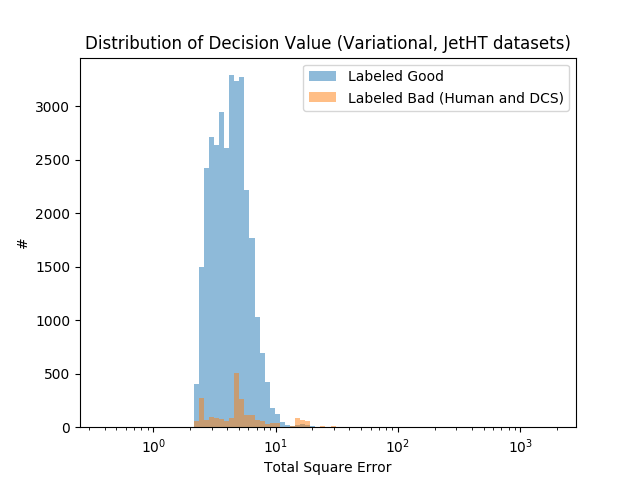
\includegraphics[width=\linewidth]{images/reco/2018/feature_2/se_dist_Variational1f2_JetHT_unlog.png}
        \caption{JetHT}
    \end{subfigure}
    \caption{Distribution of decision value}
\label{fig:2018_f2_se_dist}
\end{figure}

\subsubsection{Reconstruction Error}
Regarding Figure \ref{fig:2018_recon_error_singlemuon}, the peak around feature 50 in good LS is qglobTkN. Secondly, the couple clump around feature 80 is qglobTkChi2. The next pile is qglobTkNHits as well as last forky shape in around feature hundred dominated by qMuNCh. 

According to Figure \ref{fig:2018_recon_error_zerobias}, the residue in feature number 20 to 30 is qpVtxY. There are two huddles in bad LS where it mainly consists of qgTkPt, qgTkEta, and qgTkPhi. The clump in good LS around 70 to 80 mostly is qgTkPhi and qgTkN.

Lastly, by considering Figure \ref{fig:2018_recon_error_jetht}. Features that contain a very first peak in bad LS is qpVtxChi2. Secondly, around feature number 80 to 90 are qPFMetPt and qPFMetPhi. Lastly, there are the last two chunks of features (~120-127 and ~130-145) that behave like a noisy for both good and bad LS. Highly correlated features that show similar features (~15-35) are qpVtxX, qpVtxY, and qpVtxZ.

\begin{figure}[h!]
\centering
    \begin{subfigure}[b]{0.49\linewidth}
        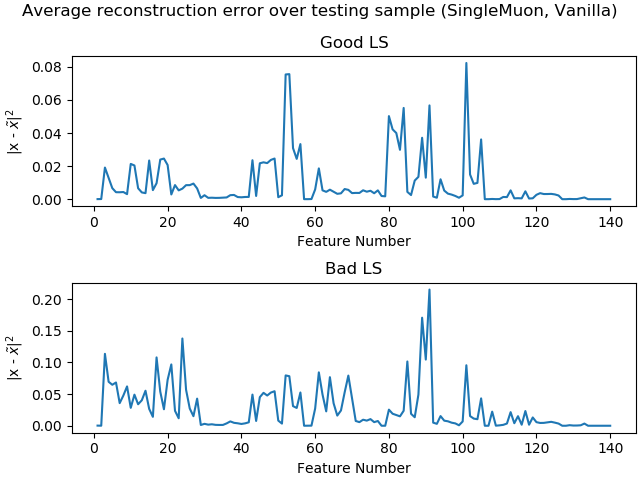
\includegraphics[width=\linewidth]{images/reco/2018/feature_2/avg_sd_Vanilla_SingleMuon_f2_1.png}
        \caption{Sum over sampling}
    \end{subfigure}
    \begin{subfigure}[b]{0.49\linewidth}
        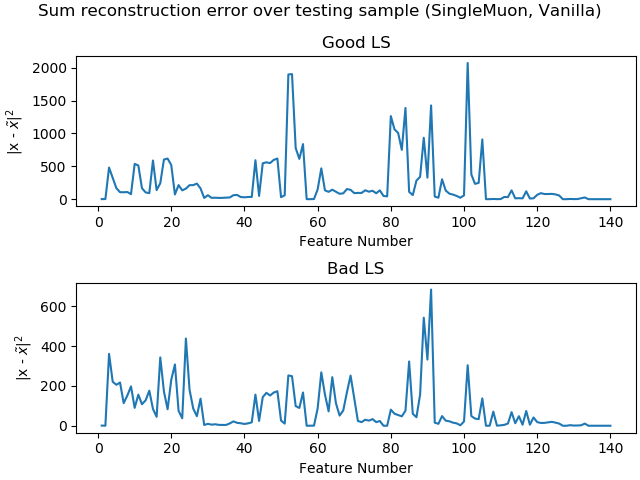
\includegraphics[width=\linewidth]{images/reco/2018/feature_2/sum_sd_Vanilla_SingleMuon_f2_1.png}
        \caption{Average over sampling}
    \end{subfigure}
    \caption{Reconstruction error of SingleMuon}
\label{fig:2018_recon_error_singlemuon}
\end{figure}

\begin{figure}[h!]
\centering
    \begin{subfigure}[b]{0.49\linewidth}
        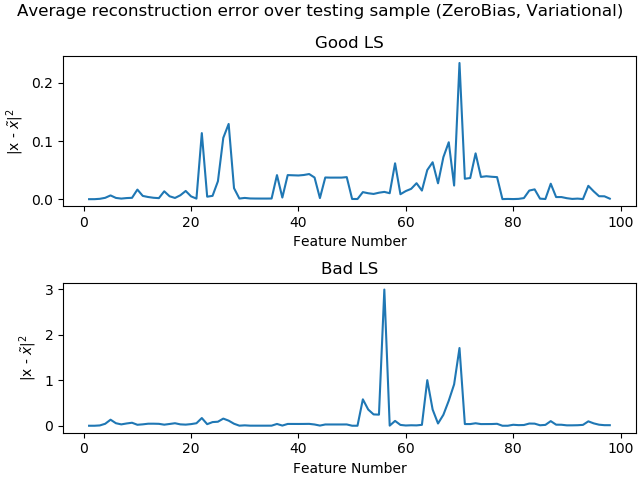
\includegraphics[width=\linewidth]{images/reco/2018/feature_2/avg_sd_Variational_ZeroBias_f2_1.png}
        \caption{Sum over sampling}
    \end{subfigure}
    \begin{subfigure}[b]{0.49\linewidth}
        \includegraphics[width=\linewidth]{images/reco/2018/feature_2/sum_sd_Variational_ZeroBias_f2_1.png}
        \caption{Average over sampling}
    \end{subfigure}
    \caption{Reconstruction error of ZeroBias}
\label{fig:2018_recon_error_zerobias}
\end{figure}

\begin{figure}[h!]
\centering
    \begin{subfigure}[b]{0.49\linewidth}
        \includegraphics[width=\linewidth]{images/reco/2018/feature_2/avg_sd_Variational_JetHT_f2_1.png}
        \caption{Sum over sampling}
    \end{subfigure}
    \begin{subfigure}[b]{0.49\linewidth}
        \includegraphics[width=\linewidth]{images/reco/2018/feature_2/sum_sd_Variational_JetHT_f2_1.png}
        \caption{Average over sampling}
    \end{subfigure}
    \caption{Reconstruction error of JetHT}
\label{fig:2018_recon_error_jetht}
\end{figure}